%!TeX spellcheck = pt_BR
\documentclass[brazil]{beamer}
%\usepackage[timeinterval=1,font=Helv]{tdclock}
\usetheme{Frankfurt}
\useoutertheme[subsection=false,footline=authortitle]{miniframes}
%\useoutertheme{shadow}


%\usepackage{beamerthemesplit}
%\usepackage{ragged2e}
%\usepackage{etoolbox}
\usepackage{hyphenat}
\usepackage{babel}
\graphicspath{{assets/}}
%\hyphenation{mate-mática recu-perar}
\usepackage[T1]{fontenc}
\usepackage{lmodern}
\usepackage[utf8x]{inputenc}
\usepackage[figurename=Imagem]{caption}
\usepackage[alf,abnt-etal-cite=2]{abntex2cite}
\usepackage{multirow}
\usepackage{tikz}
% use our .sty file for simple movie commands
\usepackage{pdfpc-commands}
%\usepackage{remreset}
%\makeatletter
%\@removefromreset{subsection}{section}
%\makeatother
%\setcounter{subsection}{1}

%\usetheme{Darmstadt}
%\setbeamerfont*{frametitle}{size=\normalsize,series=\bfseries}
%\setbeamertemplate{navigation symbols}{}
%\addtobeamertemplate{navigation symbols}{}{%
%    \usebeamerfont{footline}%
%    \usebeamercolor[fg]{footline}%
%    \hspace{1em}%
%    \insertframenumber/\inserttotalframenumber
%}
\setbeamertemplate{navigation symbols}{}
\setbeamercovered{transparent=20}
\newcommand*\oldmacro{}%
\let\oldmacro\insertshorttitle%
\renewcommand*\insertshorttitle{%
  \oldmacro\hfill%
  \insertframenumber/\inserttotalframenumber}

\setbeamertemplate{headline}
 {%
  \begin{beamercolorbox}{section in head/foot}
  \insertsectionnavigationhorizontal{\textwidth}{}{}
  \end{beamercolorbox}%
}

\AtBeginSection[]
{
  \begin{frame}
    \frametitle{Conteúdo}
    \tableofcontents[currentsection]
  \end{frame}
}


\title[Detecção inteligente de efeitos colaterais indesejáveis na Internet das coisas...]{Detecção inteligente de efeitos colaterais indesejáveis na Internet das coisas - um estudo de caso no Home Network System}
\subtitle{Apresentação de Monografia}
\author[Heron Sanches Gonçalves Pires Ferreira]{
  Heron Sanches Gonçalves Pires Ferreira
}


\institute[UFBA]{
   \\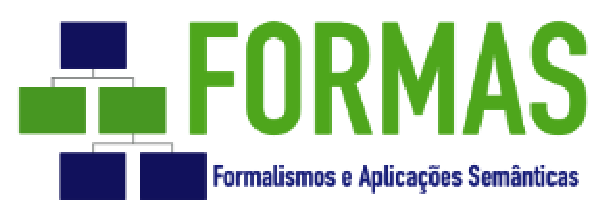
\includegraphics[width=.3\columnwidth]{logo_formas_nome}
  \\Universidade Federal da Bahia - Departamento de Ciência da Computação
  \\\textbf{Orientadora:} Profa. Dra. Daniela Barreiro Claro 
  \\\textbf{Co-Orientador:} Roberto Cerqueira Figueiredo
   \\Contato: \email{heronsanches@dcc.ufba.br} 
}

\date{31 de outubro de 2016}
%\setbeamertemplate{headline}{}
%\setbeamertemplate{background}{\hspace{.5em}\textcolor{red}{\tiny\bfseries\tdtime}}

\begin{document}
\begin{frame}
  \maketitle

  %\initclock

\end{frame}

\begin{frame}
  \frametitle{Conteúdo}
  \tableofcontents
\end{frame}

%\addtobeamertemplate{frametitle}{}{%
%\begin{tikzpicture}[remember picture,overlay]
%\node[anchor=north east,yshift=-5pt] at (current page.north east) %{\includegraphics[width=.2\columnwidth]{logo_formas}};
%\end{tikzpicture}}
\logo{\includegraphics[width=.1\columnwidth]{logo_formas}}


\section{Introdução}

\begin{frame}{Introdução}
  \begin{itemize}
    \item<1 -> A Internet está se tornando cada vez mais persistente no cotidiano \cite{Chandrakanth:2014}.
    \item<2 -> Em 2010 havia aproximadamente 1,5 bilhão de PCs conectados a Internet e mais que 1 bilhão de telefones móveis \cite{Sundmaeker:2010}.
    \item<3 ->Segundo Gartner\footnote[frame]{\url{http://www.gartner.com/newsroom/id/3165317}}, 6,4 bilhões de coisas estarão conectadas até o final de 2016 e, em 2020 esse número atingirá cerca de 20,8 bilhões.
  \end{itemize}
\end{frame}

\begin{frame}{Coisa: veículo, animal, dispositivo doméstico, pessoa, ...}
\begin{figure}[!htb] \centering 
  \centering
  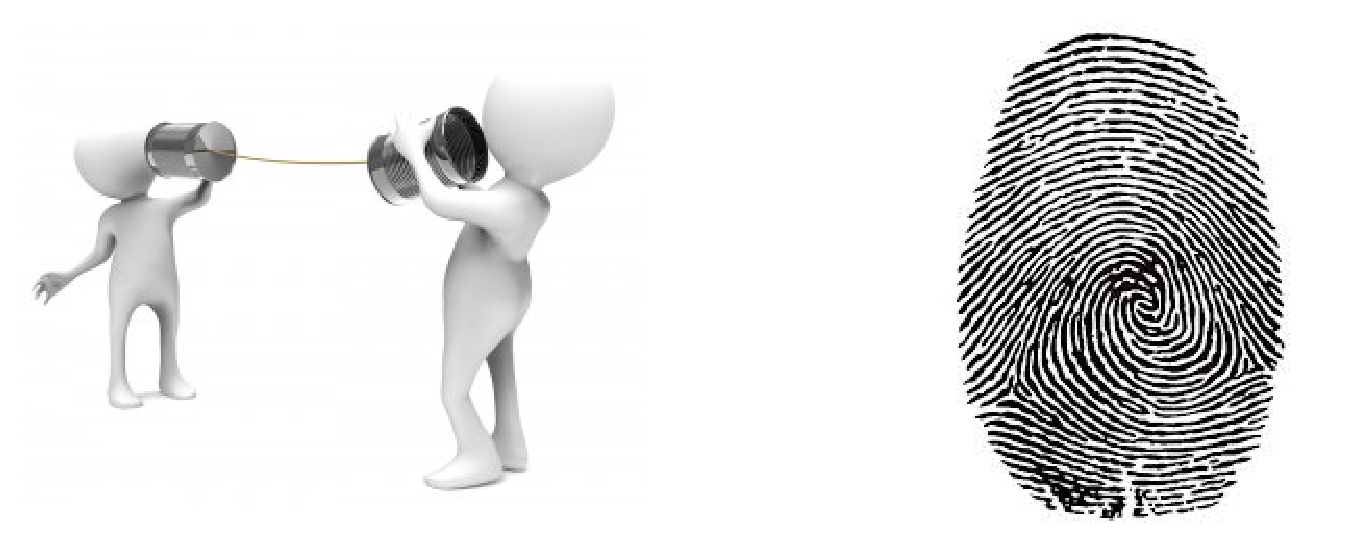
\includegraphics[width=0.8\columnwidth]{slide/coisa} 
  \caption{Baseada em \cite{Barrett}} 
  \label{fig:coisa}
\end{figure}
\end{frame}	

\begin{frame}{Internet das Coisas (IoT)}
Rede mundial de objetos unicamente endereçáveis e interconectados, seguindo os protocolos dos padrões de comunicação \cite{iot2020:2008}.
\begin{figure}[!htb] \centering 
  \centering
  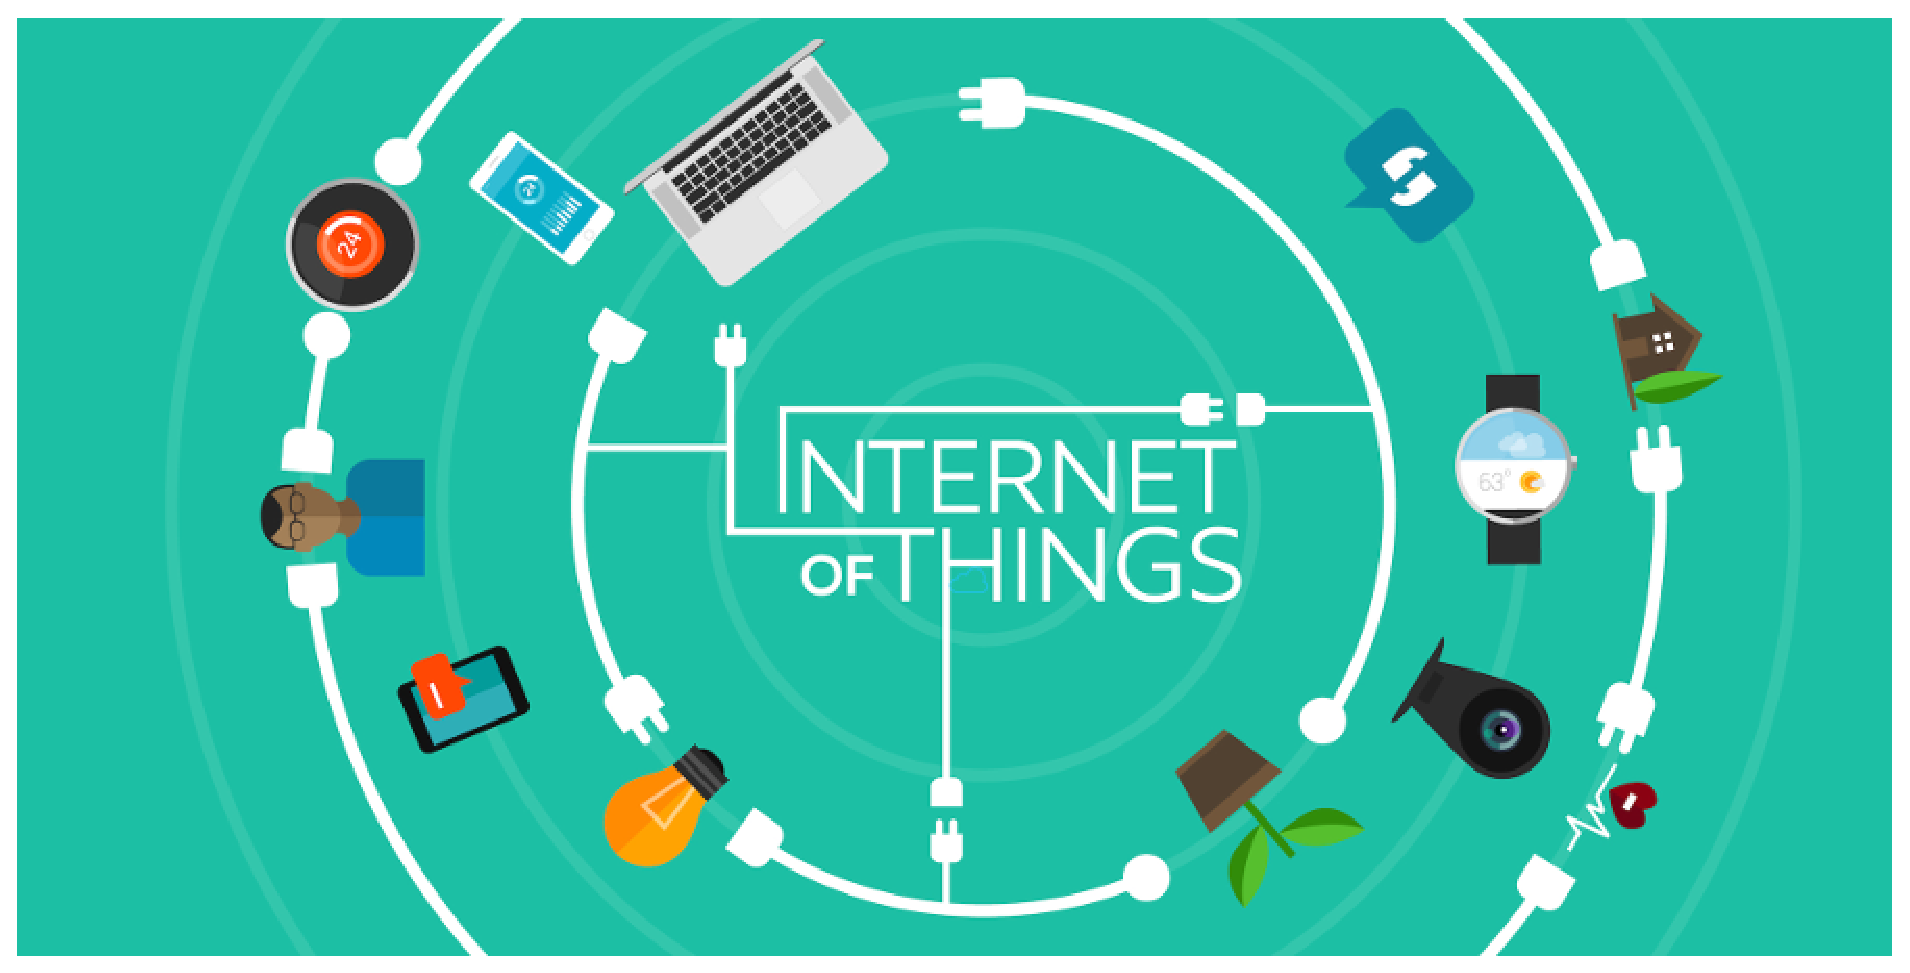
\includegraphics[width=.8\columnwidth]{slide/iot} 
  \caption{\footnote[frame]{\url{http://intca.org/2016/08/internet-of-things/}}} 
  \label{fig:iot}
\end{figure}
\end{frame}

\begin{frame}{Internet das Coisas (IoT)}
Devido ao crescente número de coisas sendo conectadas, surgem diversos desafios, a exemplo de:
  \begin{itemize}
    \item<1 -> Disponibilidade de uma interface de comunicação (acesso aos serviços e informações dos dispositivos) comum aos objetos.
    \item<2 -> Detecção e resolução de efeitos colaterais indesejáveis.
  \end{itemize}
\end{frame}

\begin{frame}{Desafios IoT: interface de comunicação padrão}
Disponibilização das coisas como serviços Web RESTFul.
  \begin{itemize}
    \item Mais leve que os serviços Web baseados em SOAP.
  \end{itemize}
\begin{figure}[!htb] \centering 
  \centering
  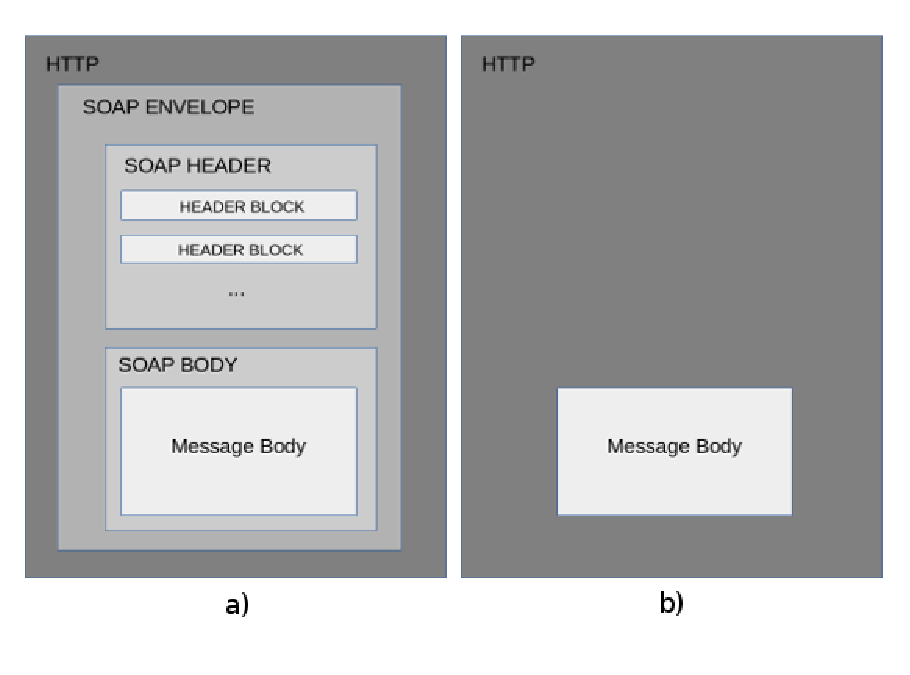
\includegraphics[width=.8\columnwidth]{slide/messages_restXsoap} 
  \caption{Baseada em \cite{Pautasso:2014}} 
  \label{fig:messages_restXsoap}
\end{figure}
\end{frame}

\begin{frame}{Desafios IoT: interface de comunicação padrão}
Disponibilização das coisas como serviços Web RESTFul.
  \begin{itemize}
    \item Mais leve que os serviços Web baseados em SOAP.
  \end{itemize}
\begin{figure}[!htb] \centering 
  \centering
  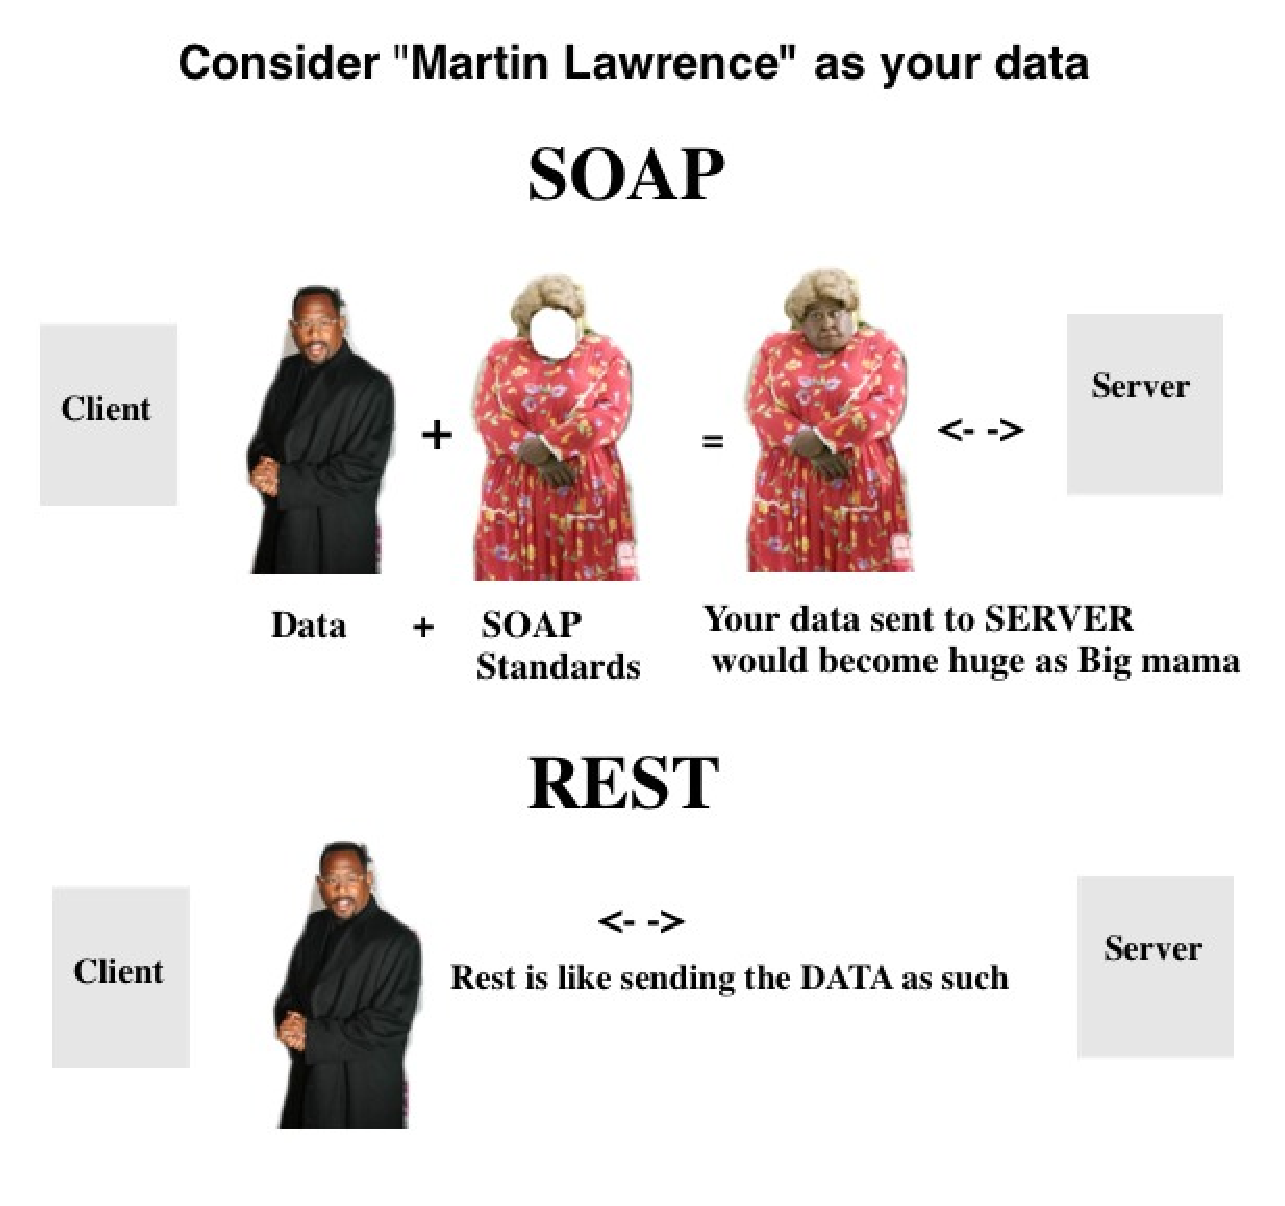
\includegraphics[width=.45\columnwidth]{slide/soapXrest_engracado} 
  \caption{\footnote[frame]{\url{http://stackoverflow.com/questions/209905/representational-state-transfer-rest-and-simple-object-access-protocol-soap}}}
  \label{fig:soapXrest_engracado}
\end{figure}
\end{frame}

\begin{frame}{Desafios IoT: detecção e resolução de efeitos colaterais indesejáveis}
Em desenvolvimento de \textit{software}, uma \alert{\textit{feature} (característica)} é um componente de adicional funcionalidade ao \textit{software} \cite{Calder:2003}, consistindo de um conjunto de requisitos logicamente relacionados e suas especificações, o qual se destina a fornecer um determinado efeito comportamental \cite{NHLABATSI:2008}
\end{frame}

\begin{frame}{Desafios IoT: detecção e resolução de efeitos colaterais indesejáveis}
Quando a \alert{composição de \textit{features}} leva a algum \alert{comportamento não esperado} - interação de características, esta pode resultar em \alert{efeitos colaterais indesejáveis}: um estado inconsistente do sistema, um sistema instável ou dados imprecisos \cite{NHLABATSI:2008}.
\end{frame}

\section{Proposta}


\section{Validação}

\section{Conclusão e trabalhos futuros}

\bibliographystyle{abntex2-alf}
\begin{frame}[allowframebreaks]{Referências}
  \bibliography{biblio}
\end{frame}

\end{document}
